\documentclass[border=15pt]{standalone}
\usepackage{tikz}
\usetikzlibrary{arrows.meta, positioning, calc, shapes.geometric}

\begin{document}

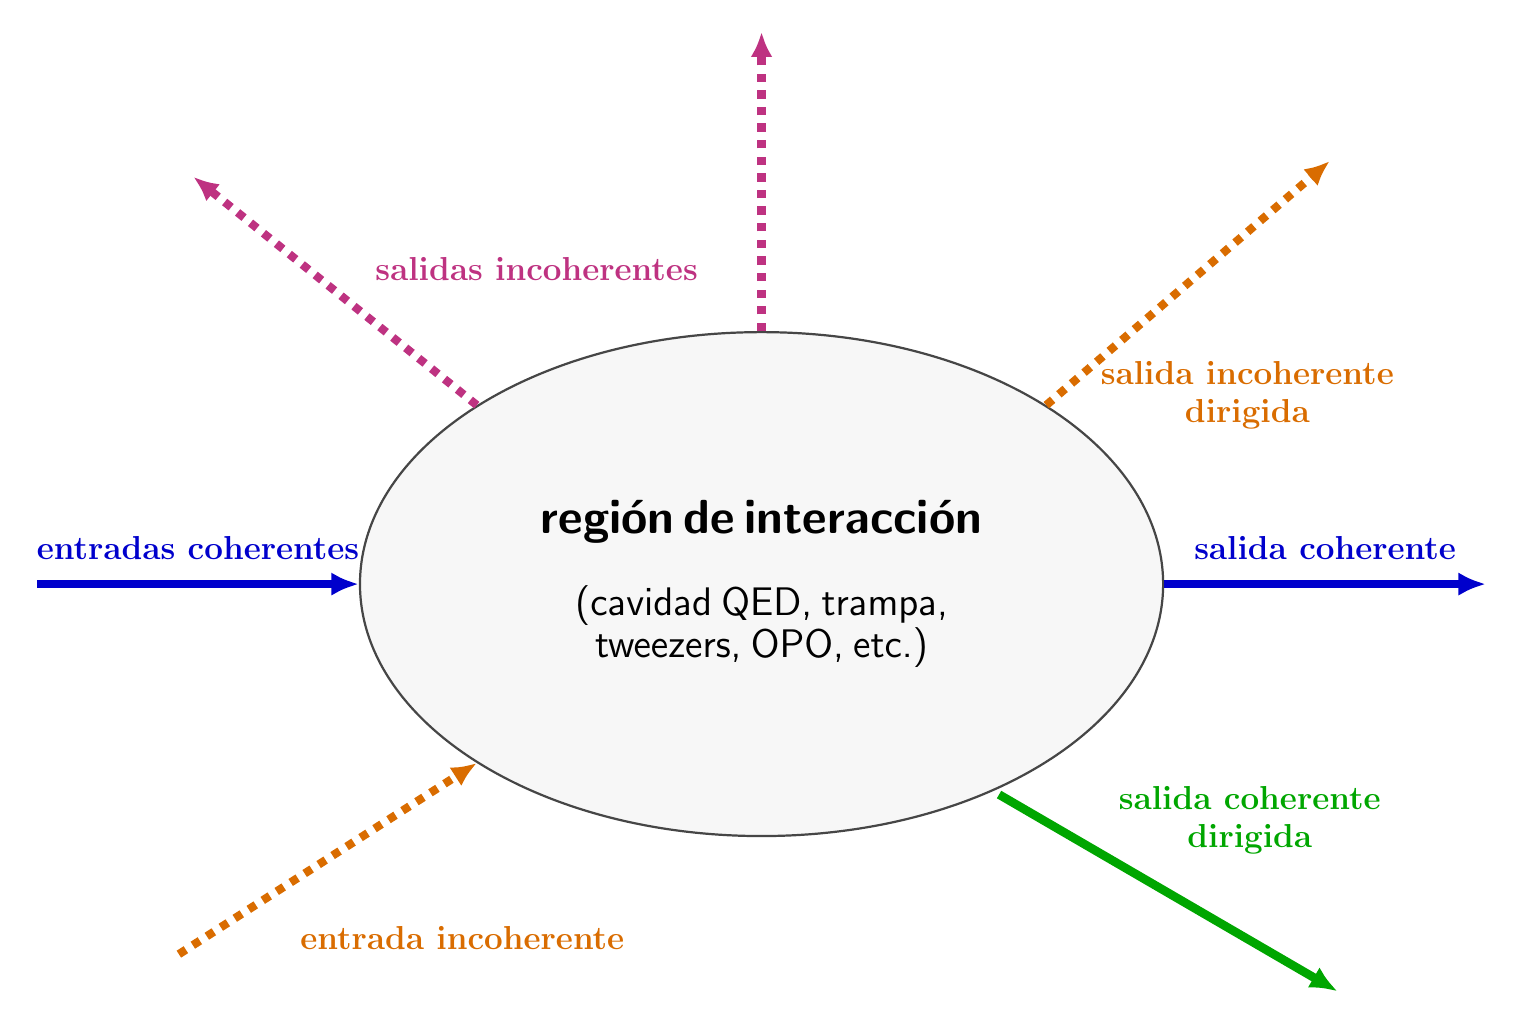
\begin{tikzpicture}[
    >=Stealth,
    font=\sffamily,
    thick,
    every label/.style = {font=\small\sffamily, inner sep=3pt},
    coh/.style = {blue!80!black, solid, line width=1.1mm, -{Latex[length=3.5mm,width=3mm]}},
    coh_dir/.style = {green!65!black, solid, line width=1.1mm, -{Latex[length=3.5mm,width=3mm]}},
    inc_in/.style = {orange!85!black, dashed, line width=1.05mm, -{Latex[length=3.2mm,width=2.8mm]}},
    inc_dir/.style = {orange!85!black, dashed, line width=1.05mm, -{Latex[length=3.2mm,width=2.8mm]}},
    inc_multi_red/.style = {magenta!75!black, dashed, line width=1.05mm, -{Latex[length=3.2mm,width=2.8mm]}},
    inc_multi_mag/.style = {magenta!75!black, dashed, line width=1.05mm, -{Latex[length=3.2mm,width=2.8mm]}},
    inc_up/.style = {magenta!75!black, dashed, line width=1.05mm, -{Latex[length=3.2mm,width=2.8mm]}},
]

% Óvalo central
\node[draw=gray!55!black, thick, fill=gray!6, ellipse,
      minimum width=10.2cm, minimum height=6.4cm, inner sep=15pt]
     (central) at (0,0) {};

% Texto central
\node[align=center, text width=8.5cm] at (central.center)
{
    \LARGE\textbf{región de interacción}\\[5mm]
    \Large (cavidad QED, trampa, tweezers, OPO, etc.)
};

% 1. Entrada coherente (izquierda)
\draw[coh]
    (-9.2,0) -- (central.west)
    node[midway, above=4pt, font=\large\bfseries]
    {entradas coherentes};

% 2. Salida coherente (derecha)
\draw[coh]
    (central.east) -- (9.2,0)
    node[midway, above=4pt, font=\large\bfseries]
    {salida coherente};

% 3. Entrada incoherente (abajo-izquierda)
% 3. Entrada incoherente (abajo-izquierda)
\draw[inc_in] (-7.4,-4.7) -- (central.south west);

\node[inc_in,font=\large\bfseries]
    at (-3.8,-4.5)
    {entrada incoherente};

    
% 4. Salida incoherente dirigida (arriba-derecha)
\draw[inc_dir] (central.north east) -- ++(3.6,3.1);
\node[inc_dir,
      anchor=south west,
      rotate=0,
      right=4pt,
      font=\large\bfseries,
      align=center]
      at (4,2.4)
      {salida incoherente\\dirigida};
% 5a. Salidas incoherentes (arriba-izquierda, rojo)
\draw[inc_multi_red] (central.north west) -- ++(-3.6,2.9);
\node[inc_multi_red, anchor=south east, rotate=0, left=4pt, font=\large\bfseries] at (-0.5,4) {salidas incoherentes};

% 5b. Salida incoherente vertical arriba (verde)
\draw[inc_up] (central.north) -- ++(0,3.8);

% 5c. Salidas incoherentes abajo-derecha (magenta)

%\draw[inc_multi_mag]
%    ($(central.south)+(0.8,-0.3)$) -- ++(3.1,-3.4)
%    node[midway, sloped, above=3pt, font=\large\bfseries]
%    {salidas incoherentes};

% 6. Salida coherente dirigida (abajo-derecha, verde sólida)
% 6. Salida coherente dirigida (abajo-derecha, verde sólida)
\draw[coh_dir]
    ($(central.south east)+(-0.6,-0.4)$) -- ++(4.3,-2.5);

\node[coh_dir,font=\large\bfseries, align=center]
    at (6.2,-3.0)
    {salida coherente\\dirigida};

\end{tikzpicture}

\end{document}